\chapter{JDBMeasure - pierwsze spojrzenie}\label{rodz:over}
Rozdział ten zawiera ogólny opis struktury benchmarku, a w szczególności omawia ideę
definicji testu poprzez tworzenie trzech modeli: bazy danych, obciążenia i testu.
Została tutaj także opisana infrastruktura benchmarku tj. podział na aplikacje
serwera i RTE.
\section{Infrastruktura}
Benchmark oparty jest o architekturę klient -- serwer (zob.~rys.~\ref{rys:infrastructure}). 
W skład benchmarku wchodzą zatem dwie aplikacje: serwera benchmarku, oraz 
klienta RTE (ang. Remote Terminal Emulator). Protokołem komunikacyjnym pomiędzy 
klientem, a serwerem jest RMI (ang. Remote Method Invocation~\cite{RMI1}). 
W celu poprawienia czytelności implementacji protokołu komunikacyjnego, 
wykorzystano wsparcie dla RMI oferowane przez bibliotekę Spring 2.0~\cite{Spring1}.

\begin{figure}[h]
\begin{center}
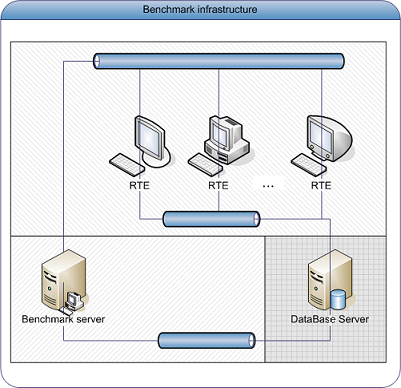
\includegraphics[width=0.6\linewidth]{figures/infrastructure.png}
\end{center}
\caption{Infrastruktura}\label{rys:infrastructure}
\end{figure}

\section{Test jako zestaw modeli}
Serwer benchmarku umożliwia ładowanie i uruchamianie testów. Każdy test składa się z trzech modeli (zob.~rys.~\ref{rys:models}):
\begin{itemize}
\item modelu bazy danych -- opisującego strukturę bazy danych, jak i populację danych w bazie przed rozpoczęciem testu,
\item modelu obciążenia -- opisującego obciążenie bazy danych. W skład tego modelu wchodzą: operacje, transakcje i użytkownicy,
\item modelu testu -- opisującego testowaną bazę danych, konfigurację połączenia do bazy, wartości parametrów skalujących 
powyższe modele, a także liczbę niezbędnych klientów RTE do przeprowadzenia testu.
\end{itemize}
\begin{figure}[h]
\begin{center}
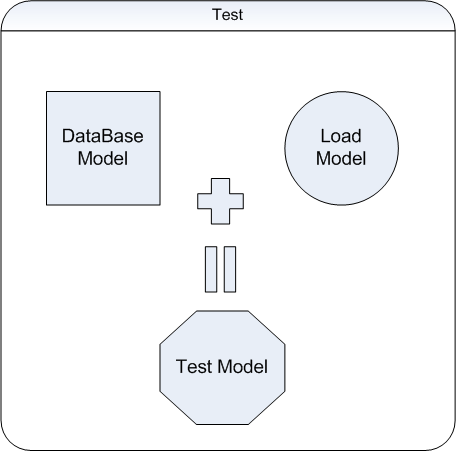
\includegraphics[width=0.4\linewidth]{figures/models.png}
\end{center}
\caption{Modele testu}\label{rys:models}
\end{figure}

\subsection{Model bazy danych}
Model bazy danych jest odpowiednikiem diagramu relacji, uzupełnionym o wartości 
liczby rekordów w poszczególnych relacjach (zob.~rys.~\ref{rys:database-model}). 
Wartości te mogą być określone względem parametru skalującego ,,n''. 
Konkretna wartość tego parametru jest określana w modelu testu. 
Liczba rekordów dla poszczególnych relacji jest wykorzystywana w procesie
generowania populacji bazy danych(zob. punkt~\ref{sect:populationgeneration}).
Warto podkreślić, iż opis zawarty w tym modelu jest niezależny od konkretnego DBMS 
(\english{Database Management System}). Formatem opisu modelu jest dokument XML,
dla którego zdefiniowano XMLSchema~\cite{XmlSchema1}, dostępną w załączniku do niniejszej pracy.
Przykładowy, uproszczony plik modelu bazy danych może wyglądać następująco:

\begin{codeblock}
<?xml version="1.0" encoding="UTF-8"?>
<database-model>
    <model-description/>
    <relations>
        <relation name="TBL_PERSON">
            <columns>
                <column name="ID" type="Long" is_id="true"/>
                <column name="FIRST_NAME" type="String(4,16)"/>
                <column name="SURNAME" type="String(4,32)"/>
                <column name="DATE_OF_BIRTH" type="Date"/>
            </columns>
        </relation>
    </relations>
    <population>
        <relation-population expression="1000*n" relation_name="TBL_PERSON"/>
    </population>
</database-model>
\end{codeblock}

W powyższym przykładzie zdefiniowano pojedynczą relację ,,TBL\_PERSON'', posiadającą
cztery atrybuty: ,,ID'', ,,FIRSTNAME'', ,,SURNAME'' oraz ,,DATE\_OF\_BIRTH''. Kolumna
,,ID'' jest kluczem głównym. Dla omawianej relacji określono niezbędną do wygenerowania 
populację początkową jako: ''1000*n'' -- oznacza to, iż liczba wygenerowanych rekordów
zależeć będzie od parametru skalującego ,,n'' i będzie od niego tysiąckrotnie większa.

\begin{figure}[h]
\begin{center}
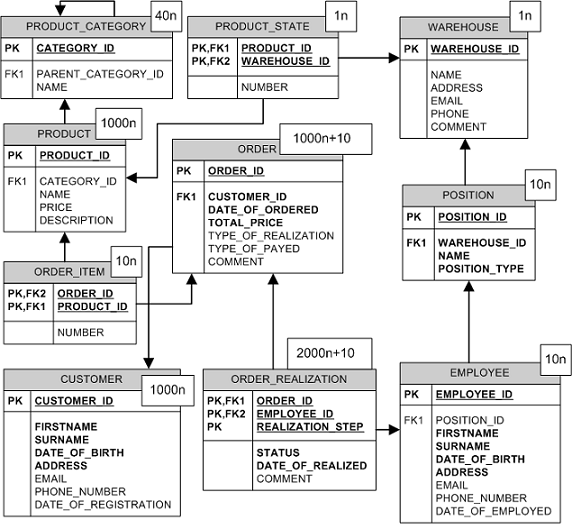
\includegraphics[width=0.9\linewidth]{figures/database-model.png}
\end{center}
\caption{Przykładowy model bazy danych}\label{rys:database-model}
\end{figure}

\subsection{Model obciążenia}
Model obciążenia(zob.~rys.~\ref{rys:load-model}) jest zmodyfikowaną wersją diagramu przypadków użycia z języka UML
(\english{Unified Modeling Language}, Ujednolicony Język Modelowania~\cite{UML1}~\cite{UML2}). Możemy tutaj wyróżnić 
użytkowników (aktorzy), a także transakcje i operacje (odpowiedniki przypadków użycia). Operacje to zwykłe operacje 
języka SQL(insert, update, delete, select).
Transakcje natomiast to zarazem transakcje w znaczeniu bazodanowym jak i odpowiedniki procesów biznesowych.
Transakcja jest uporządkowanym zbiorem krotności operacji, wchodzących w jej skład.
Istnieje możliwość określenia dla każdej transakcji minimalnej i maksymalnej liczby dla danego wystąpienia operacji.
Transakcje powodujące modyfikację zawartości bazy danych kończą się operacją ,,commit'', w przypadku wystąpienia
błędu w trakcie wykonywania którejś z operacji, transakcja kończy się operacją ,,rollback''.
Użytkownicy mogą wykonywać transakcje. Dla każdej transakcji, którą może wykonać dany użytkownik
należy podać średnią liczbę użycia na sesję. Dla każdego użytkownika podaje się czas trwania sesji,
a także liczbę użytkowników w systemie w jednostce czasu. Dany użytkownik może dziedziczyć
cechy po innym użytkowniku. Dziedziczenie może być pełne lub częściowe. Ilustruje to poniższy rysunek.

\begin{figure}[h]
\begin{center}
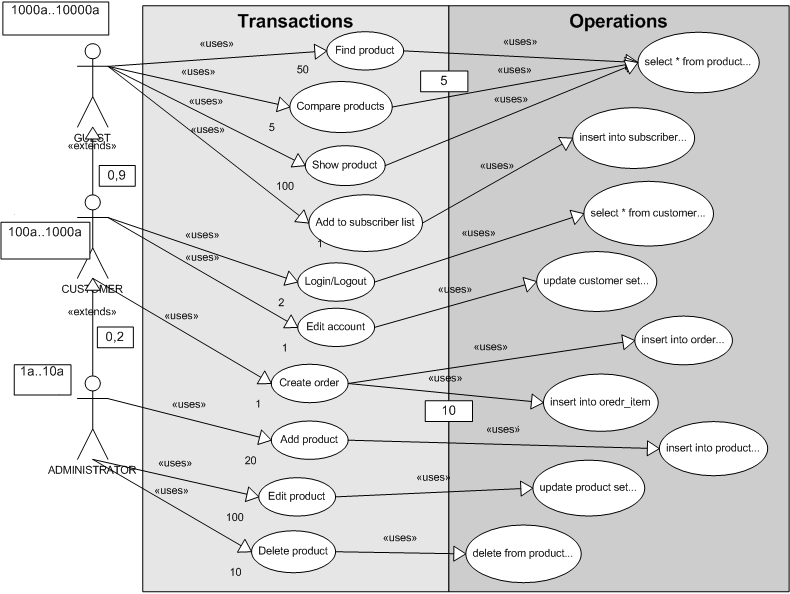
\includegraphics[width=1.0\linewidth]{figures/load-model.png}
\end{center}
\caption{Przykładowy model obciążenia}\label{rys:load-model}
\end{figure}
Widzimy tutaj min., iż transakcja ,,Create order'' składa się z dwóch typów operacji: ,,insert into order'' 
oraz ,,insert into order\_item''. Pierwsza operacja jest wykonywana w transakcji 1 raz, druga zaś 10 razy.
Użytkownik ,,Customer'' wykonuje w trakcie jednej sesji 2 transakcje ,,Login/Logout'', 1 transakcje ,,Edit account'',
oraz jedną ,,Create order''. Użytkownik ten dziedziczy również transakcje po użytkowniku ,,Guest''. Stopień dziedziczenia
określia liczba ,,0.9'' umieszczona obok strzałki od użytkownika ,,Customer'' do ,,Guest''. Oznacza to, iż 
,,Customer'' wykonuje 0.9 tych samych transakcji co ,,Guest'', czyli np. $0.9 * 100$ transakcji ,,Show product''.
W rozważanym przedziale czasu w systemie może przebywać od 100a do 1000a użytkowników typu ,,Customer''. Podczas wykonywania testów
przyjęta zostanie wartość średnia czyli 550a. 

Wszystkie powyższe cechy umożliwiają dużą elastyczność w budowie modelu obciążenia bazy danych.
Dodatkowo parametry takie, jak liczba użytkowników( parametr ,,a'') mogą być skalowane. 
Podobnie jak dla modelu bazy danych formatem opisu jest dokument XML,
dla którego zdefiniowano XMLSchema, dostępną w załączniku do niniejszej pracy.
Przykładowy, uproszczony plik modelu obciążenia może wyglądać następująco:

\begin{codeblock}
<?xml version="1.0" encoding="UTF-8"?>
<load-model>
    <description>Typowy model sklepu</description>
    <operations>
        <operation name="INSERT INTO TBL_PERSON" type="INSERT">
            <definition>INSERT INTO TBL_PERSON(FIRST_NAME,SURNAME,DATE_OF_BIRTH) 
	    		VALUES(?,?,?)</definition>
            <operation-description>Wstawienie nowego rekordu do tabeli użytkownicy</operation-description>
            <parameters>
                <parameter type="String(4,16)" number="1"/>
                <parameter type="String(4,32)" number="2"/>
                <parameter type="Date" number="3"/>
            </parameters>
        </operation>
    </operations>
    <transactions>
        <transaction name="ADD PERSON">
            <transaction-description>Add new person</transaction-description>
            <transaction-operations>
                <transaction-operation operation_name="INSERT INTO TBL_PERSON" number="1"/>
            </transaction-operations>
        </transaction>
    </transactions>
    <actors>
        <actor min_number="1*a" max_number="100*a" name="ADMIN">
            <actor-description/>
            <actor-transactions>
                <actor-transaction transaction_name="ADD PERSON" avg_call_number="100"/>
            </actor-transactions>
        </actor>
    </actors>
</load-model>
\end{codeblock}
W powyższym przykładzie zdefiniowano pojedyńczą operację ,,INSERT INTO TBL\_PERSON'',
operacja ta wstawia nowy rekord do tabeli ,,TBL\_PERSON''. Sama operacja jest typową operacją INSERT
z języka SQL, w miejscach wstawianych wartości umieszczono znaki ,,?''. Konkretne wartości są bowiem generowane
podczas tworzenia skryptów testowych. Typy generowanych wartości dla danej operacji określa się w sekcji
,,parameters''. W zamieszczonym przykładzie zdefiniowano również jedną transakcję ,,ADD PERSON''.
Transakcja ta składa się z pojedynczego wywołania operacji ,,INSERT INTO TBL\_PERSON''.
Ostatnim elementem zdefiniowanym w omawianym przykładzie jest aktor ,,ADMIN'',
reprezentuje on użytkownika typu administrator. Użytkownik ten wykonuje średnio
100 transakcji ,,ADD PERSON''.
Liczba administratorów w systemie waha się od 1*a do 100*a, gdzie ,,a'' jest parametrem skalującym dla aktorów.
Parametr ten określa się w modelu testu. Podczas testów brana jest pod uwagę średnia liczba administratorów 
czyli dla powyższego przykładu 50,5*a, przy czym po ustaleniu wartości a, liczba ta jest zaokrąglana w dół
do liczby całkowitej.

\subsection{Model testu}\label{sect:testmodel}
Model testu wiąże model bazy danych i model obciążenia. Określa on:
\begin{itemize}
\item wartości parametrów skalujących (,,a'', ,,n'', ,,c''), 
\item liczbę klientów RTE potrzebnych do wykonania testu, 
\item parametry połączenia z bazą danych, 
\item sterownik JDBC, 
\item a także, czy baza danych ma zostać usunięta po zakończeniu testu. 
\end{itemize}

To właśnie w tym modelu, poprzez specyfikacje dialektu, następuje określenie typu DBMS. 
Na podstawie zaś dialektu, w procesie przygotowywania danych, modele te są odpowiednio interpretowane.
Model ten udostępnia duże możliwości skalowalności, poszczególne parametry skalujące
mają określone zastosowanie:
\begin{itemize}
\item ,,a'' -- służy  do określania liczby użytkowników w modelu obciążenia,
\item ,,n'' -- przeznaczeniem tego parametru jest określanie liczby rekordów dla generowania populacji, w modelu bazy danych, 
\item ,,c'' -- jest parametrem wiążącym pozostałe 4 parametry, może być używany w ich definicji,
dzięki niemu można uzyskać pojedynczy parametr skalujący dla testu.
\end{itemize}
Poniżej przedstawiono przykładowy model testu:
\begin{codeblock}
<?xml version="1.0" encoding="UTF-8"?>
<test-model delete_db_after_test="false" rte_number="2" c="4" n="2000* c" a="1000*c">
	<jdbc-connection-properties>
		<property name="jdbc-library-location" value="/jar/jdbc.jar"/>
		<property name="driver_class" value="com.mysql.jdbc.Driver"/>
		<property name="dialect" value="MySQLInnoDBDialect"/>
		<property name="url" value="jdbc:mysql://localhost:3306/test"/>
		<property name="username" value="root"/>
		<property name="password" value=""/>
	</jdbc-connection-properties>
</test-model>
\end{codeblock}

W definicjach poszczególnych parametrów (,,a'', ,,n'') oraz w miejscach ich wstawiania w modelach, można
użyć operatorów ,,$+$'', ,,$-$'', ,,$*$'', ,,$:$'', ,,$^{\wedge}$'' (potęgowanie), a także funkcji ,,ln'' i ,,log'' oraz
nawiasy ,,('', ,,)''. Operacje są wykonywane w kolejności występowania od lewej do prawej tzn.
wszystkie operatory mają równy priorytet. Poprawne są zatem w definicjach modeli konstrukcje takie jak ,,$(n+((5+n)*n)):2*n$''
w miejscu dozwolonym dla parametru ,,n'' i~analogicznie dla~,,a''.
W samym modelu testu w~definicjach parametrów ,,a'' oraz~,,n'',
stosować można wyłącznie odwołania do parametru c tzn. poprawna jest definicja 
n="$2*c+1$", a niepoprawna n="$3*a$". Przykładowa definicja wszystkich parametrów
w modelu testu może wyglądać np. tak: c="1", a="2 $^{\wedge} c$", n="$100 * c + 10$".

\section{Podsumowanie}
Podział definicji testu na trzy modele, ułatwia zdefiniowanie testu. Każdy model 
ma ściśle określone przeznaczenie, razem zaś stanowią pełną definicję, 
uwzględniającą wszystkie aspekty rzeczywistego systemu opartego o współpracę z DBMS. 
Takie podejście ułatwia definiowanie testu, zmiana DBMS sprowadza się do zmiany dialektu 
i~parametrów połączenia w modelu testu. Koncepcja taka zapewnia również łatwą, 
wielokryterialną skalowalność.

